\documentclass[11pt]{beamer}
\usepackage[utf8]{inputenc}
\usepackage[T1]{fontenc}
\usepackage{lmodern}
\usepackage{amsmath}
\usepackage{amsfonts}
\usepackage{amssymb}
\usepackage{graphicx}
% \usepackage{enumitem}
\usepackage[english]{babel}
\usetheme{Rochester}

\newcommand{\icfifty}{\texttt{IC50}}

\begin{document}
	\author{Georgios Kalantzis}
	\title{Prediction of Drug-Target Bioactivities}
	\subtitle{\textit{progress on the short project}}
	%held by the  \\ \textit{Systems Approaches to Biomedical Science} CDT}
	%\logo{}
	\institute{Oxford Protein Informatics Group \\ \textit{Dept. of Statistics - University of Oxford} \vspace{2mm}\\ In collaboration with Lhasa Ltd}
	\date{}
	%\subject{}
	%\setbeamercovered{transparent}
	%\setbeamertemplate{navigation symbols}{}
	
%	\titlegraphic{
\includegraphics[width=13mm]{logo-oxfuni}\hfill %\hspace*{2.5cm}~%
%		
\includegraphics[height=10mm]{logo-opig}\hfill %\hspace{2.5cm}~%
%		
\includegraphics[width=13mm]{logo-lhasa} }
	\vfill
		\titlegraphic{
\includegraphics[width=\textwidth]{logo-SABS-full} }
\begin{frame}[plain]
	\maketitle
\end{frame}

\begin{frame}
\frametitle{Problem Definition}
\framesubtitle{Matrix Completion for Drug-Target Interactions}
The use of computational methods to enhance the efficiency of drug discovery by assessing potential new interactions.
\vspace{5mm}
\begin{enumerate}
    \item Starting point: data from previously conducted experiments
    \item Using: Machine Learning techniques and optimisation
    \item Goal: to indicate compounds that bind with proteins 
\end{enumerate}
\vspace{5mm}
\small{Billions of potential interactions exist but only a tiny fraction} is tested so far. Predicting DTI can speed-up the development of new drugs and can save resources by directing labs towards effective compounds. 
\end{frame}



\begin{frame}
\frametitle{Project Pipeline}
\framesubtitle{July 29th - October 18th}
\begin{enumerate}
\setlength\itemsep{1em}
	\item Read papers: recently published or seminal techniques
	\item Get data, curate and set-up methodology
	\item Prepare and apply some standard methods to get a baseline
	\item Develop a novel MTL approach
	\item Imputed the missing values of the matrix and evaluate
	\pause
\end{enumerate}
\begin{center}
	Tools: Python, Scikit, Keras, RDkit, bash, stackoverflow...
\end{center}
\begin{center}
    Currently using only some servers provided by OPIG.
\end{center}
\end{frame}


\begin{frame}{The dataset}
\framesubtitle{Created from scratch using ChEMBL Python API}
\begin{itemize}
    \item ChEMBL version 25
    \item Focus only on kinases \\ 
    $\hookrightarrow$ 797 in total | 155K Compounds | 721K  interactions
    \pause
    \item Select \icfifty \ (188K) and compounds with SMILES
    \item Remove duplicates and extreme values (129K)
    \pause
    \item Filter out iteratevily to produce a robust set\\
    $\hookrightarrow$ 110 proteins | 23,361 compounds | 62,656 interactions\\
    $\hookrightarrow$ On average: 569.6 | 2.68 for proteins | targets
    \pause
    \item That's only $2.438\%$ dense $\Rightarrow $ more than $97\%$ is unknown!
    \pause
    \item With a $30nM$ threshold: 21,262 active interactions
\end{itemize}
\end{frame}

\begin{frame}{Evaluation methodology}
    For maximum transparency and fairness:
    \begin{enumerate}
    \setlength\itemsep{2mm}
        \item[Test] $10\%$ of \textbf{balanced} data are used for final testing (hidden)
        \item[Train] $80\%$ randomly splitted for parameter selection and training \\
        $\hookrightarrow$ 5-fold CV with \texttt{GridSearchCV}
        \item[Valid.] $10\%$ for validation and model selection
    \end{enumerate}
    \vspace{3mm}    
    Every method is applied to the train-set with a variety of parameters, the best parametrisation is applied to the validation set and the optimal method is selected to test against the initial $10\%$.\\
    \vspace{3mm}
    \textit{\footnotesize{Currently, the validation set is $18\%$ of the total dataset.} }
\end{frame}



\begin{frame}{Related Work}
    \framesubtitle{Classification}
    The majority of published works tackle DTI within the context of binary classification: interactions are labelled as active or inactive.\\
    \vspace{5mm}
    Some representative methods are:
    \begin{itemize}
    	\item \textit{Predicting drug-target interactions using \textbf{Probabilistic Matrix Factorisation}}, Cobanoglu et al., 2013\\
    	$\hookrightarrow$ {\footnotesize A collaborative filtering approach without using any features}
    	\item \textit{Massively multitask networks for drug discovery}, Ramsundar et al., 2015\\
    	$\hookrightarrow$ {\footnotesize ECFP4 and a combination of datasets with a total of 40M points}
    \end{itemize}
\end{frame}

\begin{frame}{Related Work}
    \framesubtitle{Regression}
    Methods of this second class aim at predicting the exact value of the bioactivity, thus a more challenging problem.\\
       \vspace{5mm}
    Some representative methods are:
    \begin{itemize}
    	\item \textit{Profile-QSAR 2.0: Kinase virtual screening accuracy comparable to four-concentration IC50s for realistically novel compounds}, Martin et al., 2017 (+\textit{previous versions})\\
    	$\hookrightarrow${\footnotesize  RF with PLS and the ``challenging'' dataset of 159 kinases}
    	\item \textit{Imputation of Assay Bioactivity Data Using Deep Learning}, Whitehead et al., 2019.\\
    	$\hookrightarrow${\footnotesize  320 descriptors, 1 hidden layer $\&$ an iterative tool for incomplete data. }
    \end{itemize}
\end{frame}



\begin{frame}{My approaches}
\framesubtitle{Single Task Methods}
\begin{itemize}
	\item \icfifty \ values are transformed to $[0,1000]$ % to assist with effectiveness for regression
	\item Parameter grid searched for each method:
	\begin{itemize}
	  \item[LR:] alpha: $[1, 0.5, 0.1, 0.01]$
	  \item[RF:] $N_{est}:[10,25,50,100,150,300]$, depth: $[3,4,5,7,10,15,25]$
	  \item[NN:] $[(50),(50\times20),(50\times100),(50\times20\times10)] \ +$ \textit{logistic $+$ lbfgs}
	\end{itemize}
	\item My STL: $(2048 \times 50 \times 10 \times 1) \ + \ $\textit{relu} $+$ regularization $+$ initil.
\end{itemize}
%\begin{eqnarray}
%   \text{Random Forest} & = &0.839215 \nonumber \\
%Neural Network & = & 0.832601 \nonumber\\
%Lasso Regression & = &  0.776538 \nonumber
%\end{eqnarray}
\pause
\begin{table}

\begin{tabular}{c|c|c|c}
	Method & Training & Validation & Per target \\
	\hline
	\color{green}Lasso Regression &  0.777 & 0.321 & 0.172\\
	\color{blue}Random Forest & 0.839 & 0.357 & 0.268\\
	\color{red}Neural Network & 0.833  & 0.279 & 0.191\\
	Keras STL &  0.960 &  0.309 & 0.22 ?
\end{tabular}
\caption{Performance of each approach measured by R2 score. Training scores are averaged across each target whereas validation are averaged across each interaction. Values for last column are after excluding the extreme cases. Similar ranking wrt MSE or MAE. }
\end{table}


\end{frame}

\begin{frame}{Some results I}
%\small{R2-score per point : LR | \textbf{RF} | NN = 0.320550 | \textbf{0.357417} | 0.278828 \\
%R2-score per target: LR | \textbf{RF} | NN = 0.171555 | \textbf{0.267513} | 0.191274}
% \centering
\begin{tabular}{@{}c@{}}
      \begin{tabular}{l}
      	\small{R2-score for training per model} \\
      	\hspace{-12mm}
        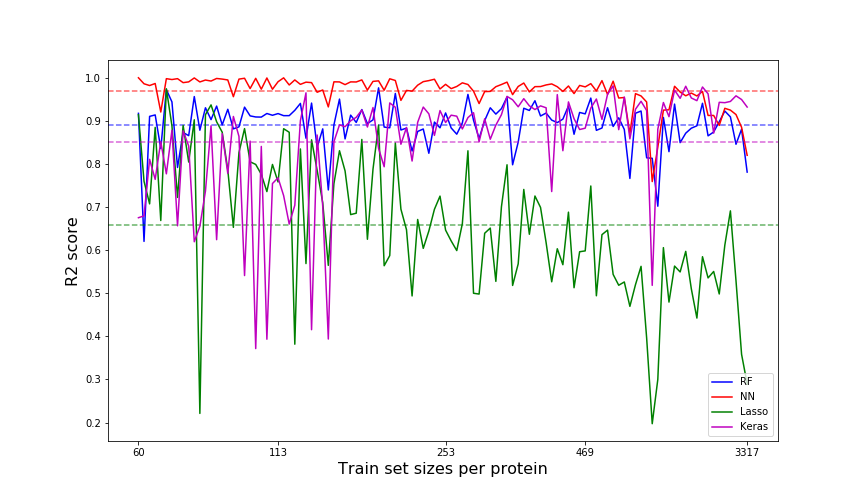
\includegraphics[width=.6\linewidth]{Train-all.png}
      \end{tabular} 
      \hspace{-10mm}
      \begin{tabular}{c}
      	\small{R2-score for validation per model} \\ 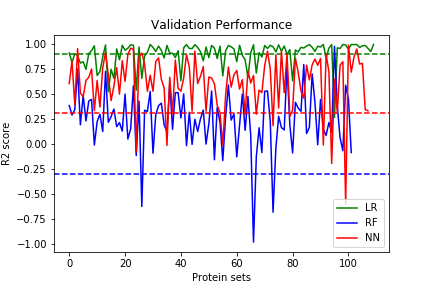
\includegraphics[width=.6\linewidth]{Valid-filtered.png}
      \end{tabular} \\
    \end{tabular}
     {\footnotesize Average performance across the 110 targets. Ordered wrt number of interacti- ons, right to left: 60 to 3317. Dashed lines show the global means. Accuracy drops for LR as the number of points is increased. All three predictors fail dra- matically for a few targets.}
\end{frame}

%\begin{frame}{Some Results II}
%	\begin{columns}[T] % align columns
%		\begin{column}{.48\textwidth}
%			\begin{figure}
%				\centering
%				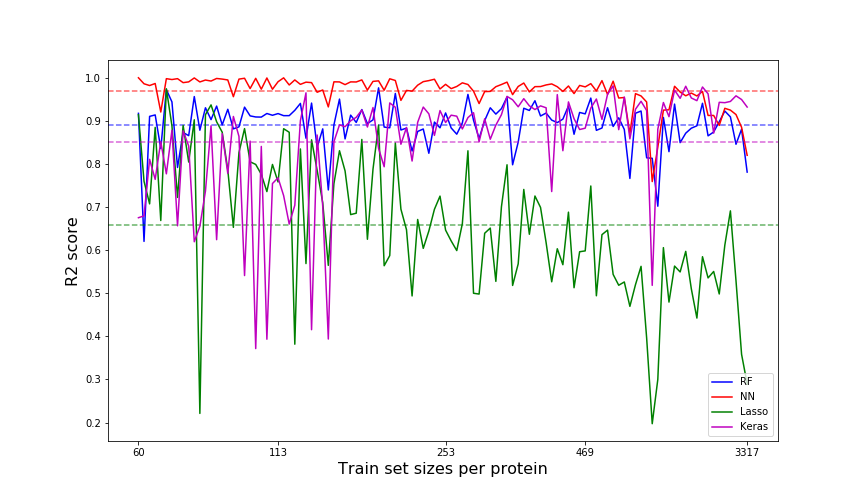
\includegraphics[width=\textwidth]{Train-all.png}
%				\caption{Caption}
%			\end{figure}
%		\end{column}%
%		\hfill%
%		\begin{column}{.48\textwidth}
%			\begin{figure}
%				\centering
%				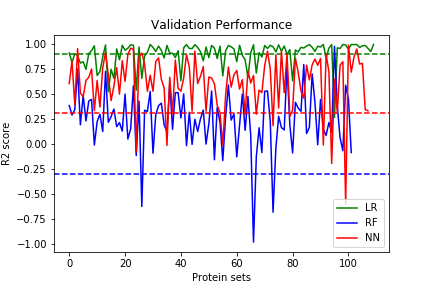
\includegraphics[width=\textwidth]{Valid-filtered.png}
%				\caption{Caption}
%			\end{figure}
%		\end{column}%
%	\end{columns}
%\end{frame}

\begin{frame}{Some Results II}
\begin{columns}[T] % align columns
    \begin{column}{.45\textwidth}
    	\vspace{3mm}
%	\vfill
	\begin{itemize}
		\item The problem is indeed tractable.
		\item There's definitely more room for improvement.
		\item Those extreme cases need extra investigation though.
		\item The range of values is crucial; standardisation does not seem to work. 
		\item Any chances for interpretation?
	\end{itemize}
	
    \end{column}%
    \hfill%
    \begin{column}{.68\textwidth}
    	\vspace{-3mm}
        \begin{figure}
            \centering
            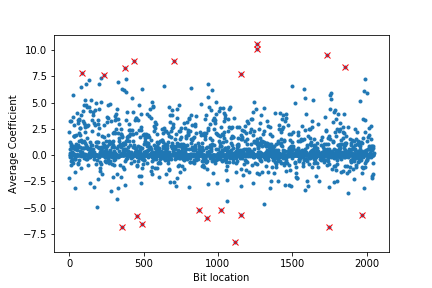
\includegraphics[width=\textwidth]{LR-FR-bits.png}
            \caption{Coefficients for ECFP bits averaged for all target-models. The vast majority is close to zero except some with consistently larger values.}
            \label{fig:my_label}
        \end{figure}
    \end{column}%
\end{columns}
\end{frame}

\begin{frame}{Multi Task Learning in Keras}
	\framesubtitle{...coming soon}
	\begin{figure}
		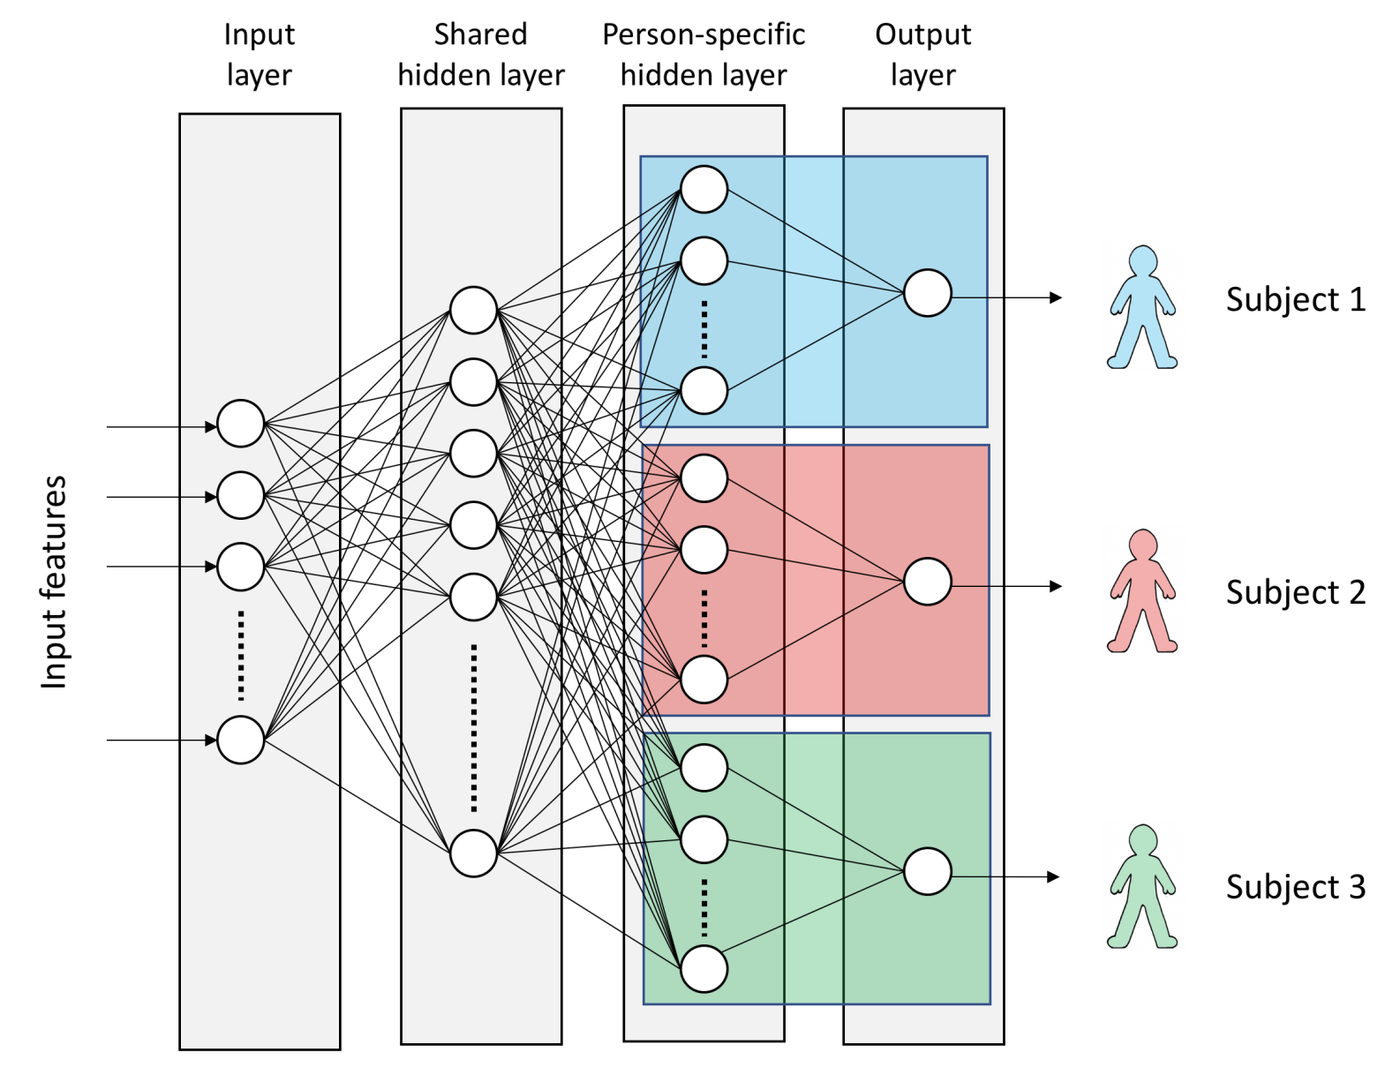
\includegraphics[width=0.9\textwidth]{MTL-3tasks-example.png}
	\end{figure}
\end{frame}

\begin{frame}
\frametitle{Future Work (\textit{immediate})}
\framesubtitle{Current progress $\sim 50\% $}
\begin{itemize}
  \setlength\itemsep{1em}
	\item So far, STL, for one target $T$ and each compound $C$: \[ \icfifty = f_{T}(\texttt{FP}(C)) \]
	\item Train/Test a MTL model with Keras, so that: \[ \icfifty = f(T,\texttt{FP}(C)) \]
	\item Use normalised/rescaled values for \icfifty 
	\item Select the optimal approach and apply it to the \textit{``159 kinases''}
	\item Redefine the test set with new/hidden compounds
	
	\item Repeat/Reproduce!
\end{itemize}
\end{frame}

\begin{frame}{Thank you}
	Please share your thoughts and any suggestions!\\
	\vspace{1em}
	Acknowledgements:
	\begin{itemize}
		\item Garrett Morris
		\item Charlotte Dean
		\item Thierry Hanser
		\item Jean-Francois Marchaland
	\end{itemize}
	\vfill
	\begin{figure}
		
\includegraphics[width=13mm]{logo-oxfuni}\hfill %\hspace*{2.5cm}~%
		
\includegraphics[height=10mm]{logo-opig}\hfill %\hspace{2.5cm}~%
		
\includegraphics[width=13mm]{logo-lhasa} 
	\end{figure}
\end{frame}
\end{document}